\documentclass{article}

\usepackage{fullpage}
\usepackage{amsmath}
\usepackage{graphicx}
\usepackage{float}

\title{Let's Search with Speedy Bois}
\date{4 December 2017}
\author{Evan Siewart \and Carter Koehler \and Michael Watts}

\begin{document}

\maketitle


\section{Citations}

\begin{itemize}

\item CSVParser
  \begin{itemize}

  \item Source: https://sourceforge.net/projects/cccsvparser/

  \item Author: talh123

  \item Last Updated: 12 April 2017

  \item Accessed: 6 November 2017
    
  \end{itemize}

\item Porter2Stemmer
  \begin{itemize}

  \item Source: https://github.com/smassung/porter2\_stemmer

  \item Author: smassung

  \item Last Updated: 19 November 2015

  \item Accessed: 2 November 2017
    
  \end{itemize}
  
\end{itemize}

\section{User Manual}

\subsection{Start Menu}

Select 1 for interactive mode (Querying, viewing statistics) or 2 for maintenance mode (Adding documents to index).

\subsection{Interactive Mode}

Type “hash” for hash table index implementation or “avl” for AVL tree implementation.

Select 1 for query search, select 2 to list top 50 most frequent words, select 3 to list number of words indexed, select 4 to list number of questions indexed, select * to exit.

\subsection{Maintenance Mode}

Press 1 to add new file to index, press 2 to clear index. If adding files, type file path followed by file name, then type * to exit when all files have been added

\subsection{Query Search}

\begin{itemize}

\item Basic usage: type in a single term to query index, type * to exit.

\item Boolean logic usage: Type “AND” or “OR” before the first term to retrieve questions related to both or either terms respectively (Ex. AND java C++). If “NOT” is included at the end, questions containing all terms following “NOT” will be excluded (Ex. OR java C++ NOT python).

\item Bracket term usage: Use square brackets to query two-word terms. Bracketed terms longer than two words will be rejected (Ex. [computer science]).

\item If no results are found “No results found” will be displayed.

\item If results are found, the 15 most relevant results will be displayed. If less than 15 results are found, all results will be displayed, sorted by relevancy.

\item To view details of a result, type corresponding number.

\item Type Y to query another term, or N to exit.
  
\end{itemize}

\section{UML Diagrams}

\begin{figure}[H]
  \centering
  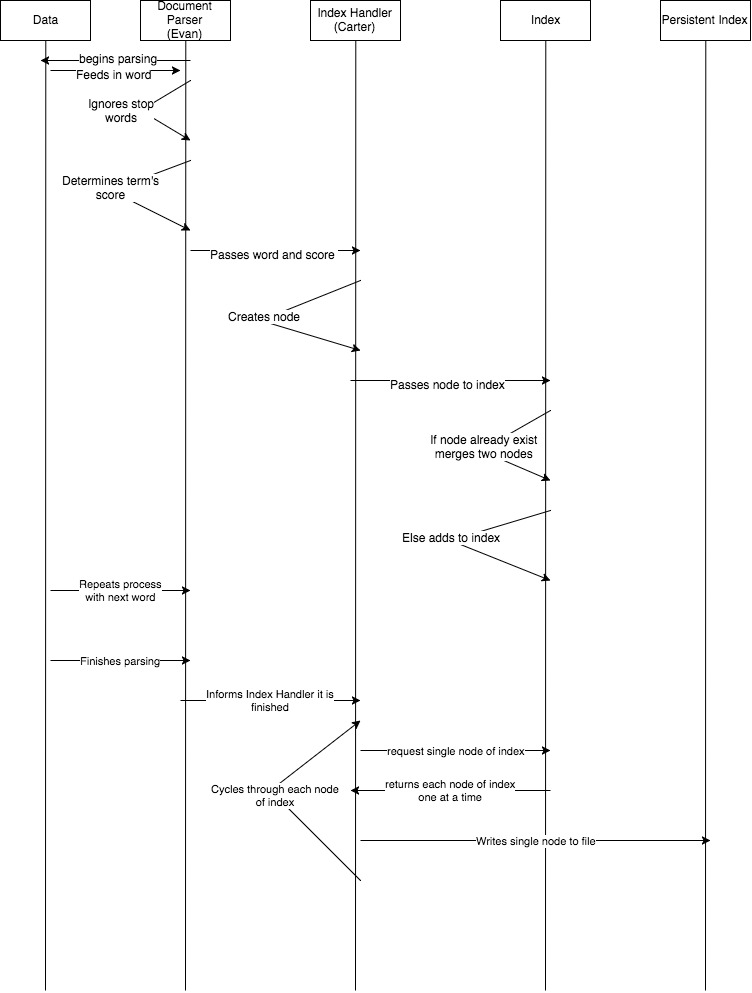
\includegraphics[width=\linewidth]{DS_Maintenance.jpg}
  \caption{UML diagram for the search engine running under maintenance mode.}
\end{figure}

\begin{figure}[H]
  \centering
  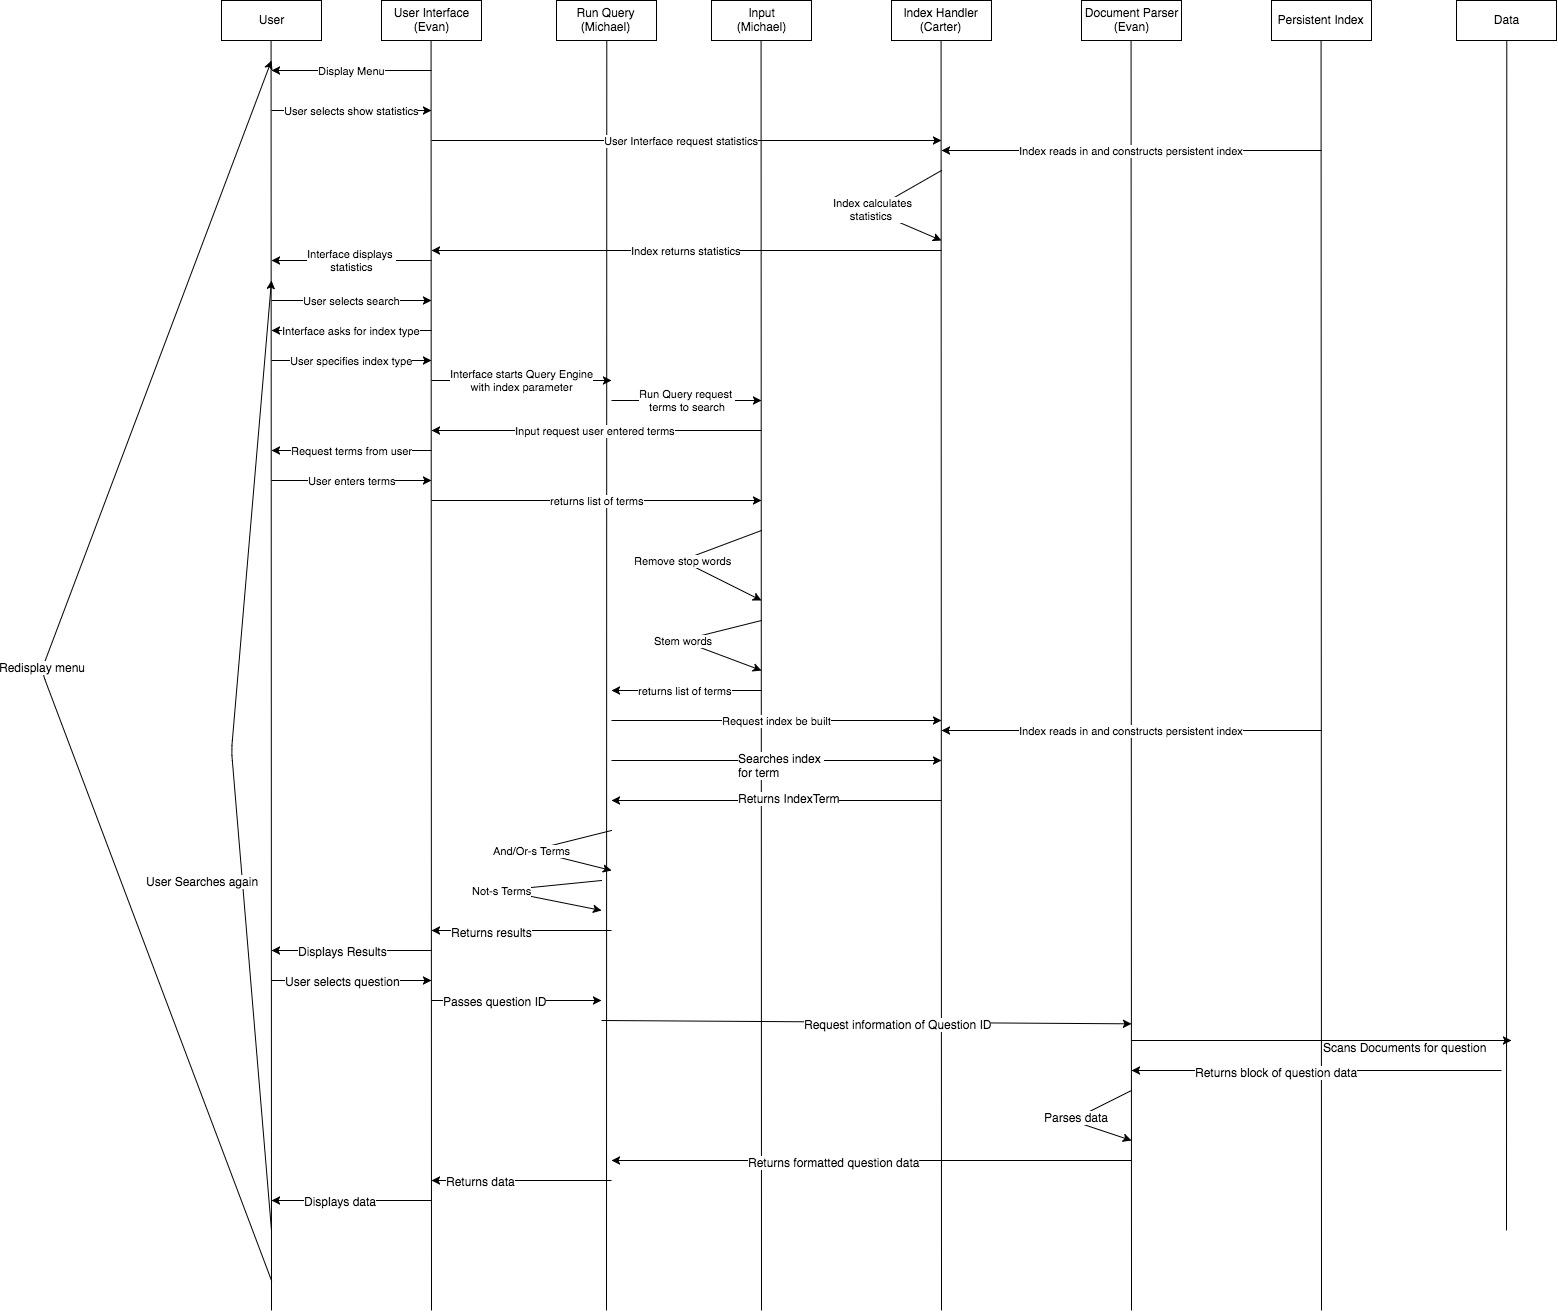
\includegraphics[width=\linewidth]{DS_Query.jpg}
  \caption{UML diagram for the search engine running under interactive mode.}
\end{figure}

\section{Comparison of Data Structures}

\subsection{Insertions}

\begin{figure}[H]
  \centering
  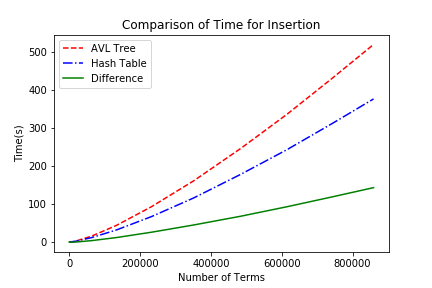
\includegraphics[width=\linewidth]{comparison-insert.png}
  \caption{Comparison of runtimes for insertions into Hash Table and AVL Tree. Times are cumulative and include time for parsing files.}
\end{figure}

Based on the data for insertions, we can see that the hash table handles insertions quite a bit faster than the AVL tree. This is because the complexity of insertions into a hash table is constant with respect to time ($O(1)$, with some accounting for nodes increasing in size), while AVL trees have time complexity $O(lgn)$. This means that, informally, inserting $n$ objects into a hash table should grow linearly with $n$, while it should grow like $n*log_2n$ for the AVL tree, both of which appear to be borne out by the data.

\subsection{Searches}

\begin{figure}[H]
  \centering
  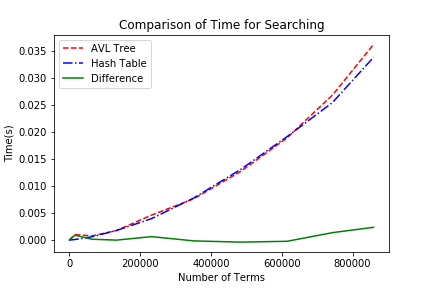
\includegraphics[width=\linewidth]{comparison-search.png}
  \caption{Comparison of runtimes for searches in Hash Table and AVL Tree of given size. Times are not cumulative.}
\end{figure}

Here, we see something somewhat unexpected. Searching in the hash table takes about as much time as does searching in the AVL tree. Again, the complexity of searching in a hash table ought to be constant in time with some slight growth over long periods of time, and the AVL tree should be logarithmic. However, these times are sufficiently small that larger trends may not be visible at this scale.

In this regard, the AVL tree and hash table are roughly comparable.

\end{document}